\documentclass{standalone}
\usepackage{tikz}
\usetikzlibrary{patterns, positioning}
\usepackage[sfdefault]{ClearSans} %% option 'sfdefault' activates Clear Sans as the default text font
\usepackage[T1]{fontenc}

\begin{document}
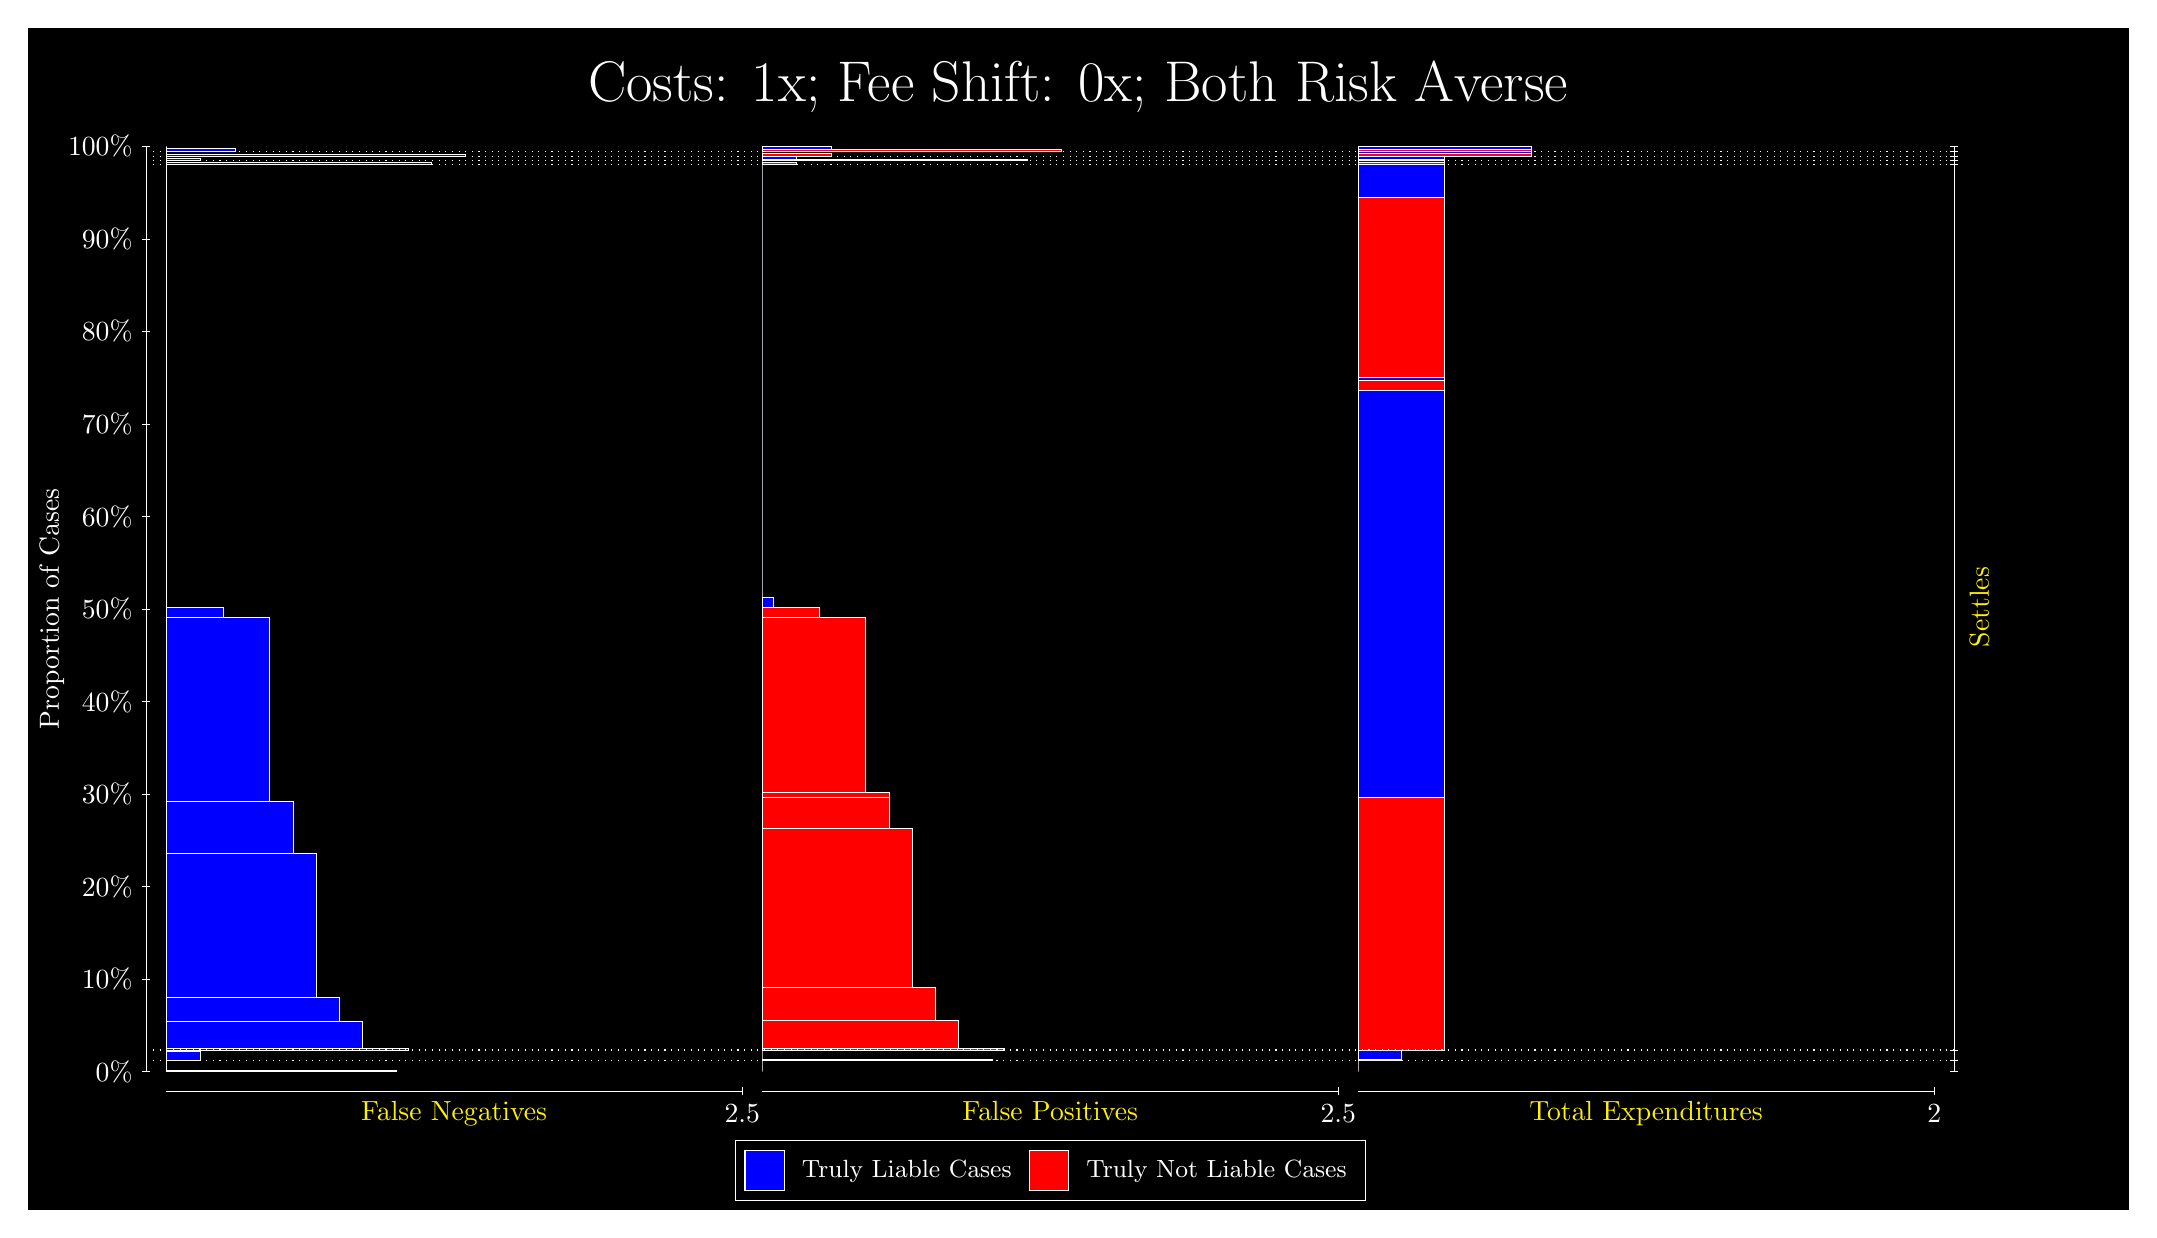
\begin{tikzpicture}
\draw[fill=black] (0,0) rectangle (26.667,15);
\draw[text=white] (0,13.5) rectangle (26.667,15) node[midway] {\huge Costs: 1x; Fee Shift: 0x; Both Risk Averse};
\draw[white, very thin] (1.5,1.75) -- (1.5,13.5);
\node[rotate=90, text=white, anchor=center] at (0.3, 7.625) {Proportion of Cases};
\draw[white, very thin] (1.45,1.75) -- (1.55,1.75);
\node[text=white, anchor=east] at (1.45, 1.75) {0\%};
\draw[white, very thin] (1.45,2.925) -- (1.55,2.925);
\node[text=white, anchor=east] at (1.45, 2.925) {10\%};
\draw[white, very thin] (1.45,4.1) -- (1.55,4.1);
\node[text=white, anchor=east] at (1.45, 4.1) {20\%};
\draw[white, very thin] (1.45,5.275) -- (1.55,5.275);
\node[text=white, anchor=east] at (1.45, 5.275) {30\%};
\draw[white, very thin] (1.45,6.45) -- (1.55,6.45);
\node[text=white, anchor=east] at (1.45, 6.45) {40\%};
\draw[white, very thin] (1.45,7.625) -- (1.55,7.625);
\node[text=white, anchor=east] at (1.45, 7.625) {50\%};
\draw[white, very thin] (1.45,8.8) -- (1.55,8.8);
\node[text=white, anchor=east] at (1.45, 8.8) {60\%};
\draw[white, very thin] (1.45,9.975) -- (1.55,9.975);
\node[text=white, anchor=east] at (1.45, 9.975) {70\%};
\draw[white, very thin] (1.45,11.15) -- (1.55,11.15);
\node[text=white, anchor=east] at (1.45, 11.15) {80\%};
\draw[white, very thin] (1.45,12.325) -- (1.55,12.325);
\node[text=white, anchor=east] at (1.45, 12.325) {90\%};
\draw[white, very thin] (1.45,13.5) -- (1.55,13.5);
\node[text=white, anchor=east] at (1.45, 13.5) {100\%};

\draw[white, very thin] (24.457,1.75) -- (24.457,13.5);
\draw[white, very thin] (24.407,1.75) -- (24.507,1.75);
\node[anchor=west] at (24.407, 1.75) {};
\draw[white, very thin] (24.407,1.8866) -- (24.507,1.8866);
\node[anchor=west] at (24.407, 1.8866) {};
\draw[white, very thin] (24.407,2.0233) -- (24.507,2.0233);
\node[anchor=west] at (24.407, 2.0233) {};
\draw[white, very thin] (24.407,13.274) -- (24.507,13.274);
\node[anchor=west] at (24.407, 13.274) {};
\draw[white, very thin] (24.407,13.32) -- (24.507,13.32);
\node[anchor=west] at (24.407, 13.32) {};
\draw[white, very thin] (24.407,13.371) -- (24.507,13.371);
\node[anchor=west] at (24.407, 13.371) {};
\draw[white, very thin] (24.407,13.436) -- (24.507,13.436);
\node[anchor=west] at (24.407, 13.436) {};
\draw[white, very thin] (24.407,13.5) -- (24.507,13.5);
\node[anchor=west] at (24.407, 13.5) {};

\draw[white, very thin, fill=blue] (1.75,1.75) rectangle (4.6775,1.7644);
\draw[white, very thin, fill=red] (1.75,1.7644) rectangle (1.75,1.8866);
\draw[white, very thin, fill=blue] (1.75,1.8866) rectangle (2.1891,2.0089);
\draw[white, very thin, fill=red] (1.75,2.0089) rectangle (1.75,2.0233);
\draw[white, very thin, fill=blue] (1.75,2.0233) rectangle (4.8239,2.0512);
\draw[white, very thin, fill=blue] (1.75,2.0512) rectangle (4.2384,2.3905);
\draw[white, very thin, fill=blue] (1.75,2.3905) rectangle (3.9457,2.6986);
\draw[white, very thin, fill=blue] (1.75,2.6986) rectangle (3.6529,4.5157);
\draw[white, very thin, fill=blue] (1.75,4.5157) rectangle (3.3602,5.179);
\draw[white, very thin, fill=blue] (1.75,5.179) rectangle (3.0674,7.5203);
\draw[white, very thin, fill=blue] (1.75,7.5203) rectangle (2.4819,7.6477);
\draw[white, very thin, fill=red] (1.75,7.6477) rectangle (1.75,13.274);
\draw[white, very thin, fill=blue] (1.75,13.274) rectangle (5.1167,13.293);
\draw[white, very thin, fill=red] (1.75,13.293) rectangle (1.75,13.32);
\draw[white, very thin, fill=blue] (1.75,13.32) rectangle (2.1891,13.35);
\draw[white, very thin, fill=red] (1.75,13.35) rectangle (1.75,13.371);
\draw[white, very thin, fill=blue] (1.75,13.371) rectangle (5.5558,13.393);
\draw[white, very thin, fill=red] (1.75,13.393) rectangle (1.75,13.436);
\draw[white, very thin, fill=blue] (1.75,13.436) rectangle (2.6283,13.478);
\draw[white, very thin, fill=red] (1.75,13.478) rectangle (1.75,13.5);
\draw[white, very thin, fill=red] (9.3189,1.75) rectangle (9.3189,1.8723);
\draw[white, very thin, fill=blue] (9.3189,1.8723) rectangle (9.3189,1.8866);
\draw[white, very thin, fill=red] (9.3189,1.8866) rectangle (12.246,1.901);
\draw[white, very thin, fill=blue] (9.3189,1.901) rectangle (9.3189,2.0233);
\draw[white, very thin, fill=red] (9.3189,2.0233) rectangle (12.393,2.0512);
\draw[white, very thin, fill=red] (9.3189,2.0512) rectangle (11.807,2.4027);
\draw[white, very thin, fill=red] (9.3189,2.4027) rectangle (11.515,2.8235);
\draw[white, very thin, fill=red] (9.3189,2.8235) rectangle (11.222,4.8346);
\draw[white, very thin, fill=red] (9.3189,4.8346) rectangle (10.929,5.2321);
\draw[white, very thin, fill=red] (9.3189,5.2321) rectangle (10.929,5.2992);
\draw[white, very thin, fill=red] (9.3189,5.2992) rectangle (10.636,7.5225);
\draw[white, very thin, fill=red] (9.3189,7.5225) rectangle (10.051,7.6499);
\draw[white, very thin, fill=blue] (9.3189,7.6499) rectangle (9.4652,7.7773);
\draw[white, very thin, fill=blue] (9.3189,7.7773) rectangle (9.3189,13.274);
\draw[white, very thin, fill=red] (9.3189,13.274) rectangle (9.758,13.301);
\draw[white, very thin, fill=blue] (9.3189,13.301) rectangle (9.3189,13.32);
\draw[white, very thin, fill=red] (9.3189,13.32) rectangle (12.686,13.341);
\draw[white, very thin, fill=blue] (9.3189,13.341) rectangle (9.758,13.371);
\draw[white, very thin, fill=red] (9.3189,13.371) rectangle (10.197,13.413);
\draw[white, very thin, fill=blue] (9.3189,13.413) rectangle (9.3189,13.436);
\draw[white, very thin, fill=red] (9.3189,13.436) rectangle (13.125,13.458);
\draw[white, very thin, fill=blue] (9.3189,13.458) rectangle (10.197,13.5);
\draw[white, very thin, fill=red] (16.888,1.75) rectangle (16.888,1.8723);
\draw[white, very thin, fill=blue] (16.888,1.8723) rectangle (16.888,1.8866);
\draw[white, very thin, fill=red] (16.888,1.8866) rectangle (17.437,1.901);
\draw[white, very thin, fill=blue] (16.888,1.901) rectangle (17.437,2.0233);
\draw[white, very thin, fill=red] (16.888,2.0233) rectangle (17.986,5.2321);
\draw[white, very thin, fill=blue] (16.888,5.2321) rectangle (17.986,10.407);
\draw[white, very thin, fill=red] (16.888,10.407) rectangle (17.986,10.534);
\draw[white, very thin, fill=blue] (16.888,10.534) rectangle (17.986,10.562);
\draw[white, very thin, fill=red] (16.888,10.562) rectangle (17.986,12.852);
\draw[white, very thin, fill=blue] (16.888,12.852) rectangle (17.986,13.274);
\draw[white, very thin, fill=red] (16.888,13.274) rectangle (17.986,13.301);
\draw[white, very thin, fill=blue] (16.888,13.301) rectangle (17.986,13.32);
\draw[white, very thin, fill=red] (16.888,13.32) rectangle (17.986,13.341);
\draw[white, very thin, fill=blue] (16.888,13.341) rectangle (17.986,13.371);
\draw[white, very thin, fill=red] (16.888,13.371) rectangle (19.083,13.413);
\draw[white, very thin, fill=blue] (16.888,13.413) rectangle (19.083,13.436);
\draw[white, very thin, fill=red] (16.888,13.436) rectangle (19.083,13.458);
\draw[white, very thin, fill=blue] (16.888,13.458) rectangle (19.083,13.5);
\draw[white, dotted] (1.5,1.8866) -- (24.457,1.8866);
\draw[white, dotted] (1.5,2.0233) -- (24.457,2.0233);
\draw[white, dotted] (1.5,13.274) -- (24.457,13.274);
\draw[white, dotted] (1.5,13.32) -- (24.457,13.32);
\draw[white, dotted] (1.5,13.371) -- (24.457,13.371);
\draw[white, dotted] (1.5,13.436) -- (24.457,13.436);
\draw[white, very thin] (1.75,1.5) -- (9.0689,1.5);
\node[text=yellow, anchor=north] at (5.4094, 1.5) {False Negatives};
\draw[white, very thin] (9.0689,1.45) -- (9.0689,1.55);
\node[text=white, anchor=north] at (9.0689, 1.45) {2.5};

\draw[white, very thin] (9.3189,1.5) -- (16.638,1.5);
\node[text=yellow, anchor=north] at (12.978, 1.5) {False Positives};
\draw[white, very thin] (16.638,1.45) -- (16.638,1.55);
\node[text=white, anchor=north] at (16.638, 1.45) {2.5};

\draw[white, very thin] (16.888,1.5) -- (24.207,1.5);
\node[text=yellow, anchor=north] at (20.547, 1.5) {Total Expenditures};
\draw[white, very thin] (24.207,1.45) -- (24.207,1.55);
\node[text=white, anchor=north] at (24.207, 1.45) {2};



\node[text=yellow, centered, rotate=90] at (24.777, 7.6488) {Settles};





\draw (12.978300999999998,1.5) node[draw=none] (baseCoordinate) {};
\begin{scope}[align=center]
        \matrix[scale=0.5, draw=white, below=0.5cm of baseCoordinate, nodes={draw}, column sep=0.1cm]{
            \node[rectangle, draw, minimum width=0.5cm, minimum height=0.5cm, fill=blue] {}; &
            \node[draw=none, font=\small, text=white] (B) {Truly Liable Cases}; &
            \node[rectangle, draw, minimum width=0.5cm, minimum height=0.5cm, fill=red] {}; &
            \node[draw=none, font=\small, text=white] (B) {Truly Not Liable Cases}; \\
            };
\end{scope}

\end{tikzpicture}
\end{document}